%The lack of standards and the need for a better understanding of mobile storage systems can easily be seen by surveying through standardized and well-known mobile database system benchmarks, which in fact non-existent~\cite{kennedy2015pocket}, while traditional database systems have a few dependable benchmarks~\cite{council2008tpch, council2010tpcc}.
%Also, traditional database systems are usually managed by professional database administrators who tune-up the databases according to changing workloads while smartphone databases work with predetermined indexes and are not subject to tuning up depending on the workload they are experiencing.
%Although there were some efforts to measure the performance of SQLite and Android devices under different workloads~\cite{kim2012androbench}, these benchmarks do not specify the bottlenecks, how and where the tune ups should be performed or they do not provide any information specific to the app performance.

%While the most visible parameter of data is its volume, it is not the only characteristic that matters.
%In fact, there are four key characteristics about data~\cite{ORCL-BIGDATA-519135}:
%\begin{itemize}
%	\item \textbf{Volume.} The most intuitive characteristic about data is the amount of data itself. In fact, it is the sheer amount of data that we generate and process these days that calls for a better approach to data management. It is one of the driving forces behind this work.
%	\item \textbf{Velocity.} Velocity refers to the idea of the amount of data flowing through an interface in unit time. 
%	\item \textbf{Variety.} Traditional data formats were relatively well defined by a data schema and changed slowly. In contrast, modern data formats change at a dizzying rate. This is referred as variety in data.
%	\item \textbf{Value.} The value of data varies significantly. The challenge in drawing insights from data is identifying what is valuable and then transforming and extracting the data for analysis.
%\end{itemize}

%Database servers and web applications experience a workload that is not typical in smartphones.
%The majority of these servers form the backbone of an application.
%In most cases, they store the business data to support OLTP and OLAP operations.
%The data volumes may range from medium to high amounts for systems with a large concurrent user base.
%The data velocity also grows in proportion to the number of concurrent users.

%The usage pattern of databases in smartphones differs significantly from the above-mentioned ideas.
%Most modern day smartphones rely on some kind of a web service to help a mobile application deliver the desired functionality to the user.
%This introduces various new application design considerations.
%Mobile users must be able to work without a network connection due to poor or nonexistent connection.
%In that case, a mobile database serves as a cache to hold recently accessed data and transactions so that they are not lost due to connection failure.
%In many cases, users might not expect live data during connection failures; only recently modified data.
%Update of recent changes and downloading of live data can be deferred until connection is restored.

%Mobile computing devices tend to have slower CPUs and limited battery life.
%The luxury of having a cluster of powerful computers to deploy a database is just not there.
%Also, the fact that battery power is scarce drives the case further to achieve high resource utilization.

%It is a common practice among smartphone users to have multiple devices.
%Most smartphones have an authentication system which is powered by an email account which is accessed in other devices too.
%In most cases, the user has at least one more device or a web service that needs to sync with the smartphone.
%This leads to occasional synchronization activities that occur between different devices and a centralized data store.
%Often, this activity happens in the background so that the user is not blocked from using other functions on a smartphone. 

%The PocketData dataset \cite{kennedy2015pocket} provides handset-based data directly collected from smartphones for multiple users.
%User sessions in context of smartphones might not be similar to a session on other more traditional computing devices like PCs.
%Typically, an end user would use their smartphones in multiple small intervals of time through a day.
%These `bursts of activity' can be referred to as session.
%In context of a single mobile application, the user would access multiple logical transactions in these bursts of activity.
%Intuitively, a user session is quite straightforward to understand, but its technical  aspects require defining.
%Some smartphone usage studies define a session as the time period where the smartphone's screen is active~\cite{soikkeli2011diversity}.
%Smartphone usage is dominated by usage of the applications that the smartphone has to offer.
%Thus, the idea of a smartphone usage session can be reduced to an application usage session.
%This is relevant to us because we aim to study the interaction with the smartphone database through understanding a single application.

%\subsection{Mobile Workload Characteristics}

The usage pattern of databases in smartphones differs significantly from the traditional database server and web application workloads.
Most modern day smartphones typically rely on a web service to help a mobile application deliver the desired functionality of the application to the user, as opposed to keeping the actual data in the database.
%This introduces various new application design considerations.
%Mobile users must be able to work without a network connection due to poor or nonexistent connection.
Thus, a mobile database typically serves as a cache to hold recently accessed data to be used in case of a connection failure, and data required for the business logic of the mobile application.
This enables the application to defer getting updates of recent changes, and downloading of live data until connection is restored.
Also, this helps asynchronously fetching data from the web services while still being able to show the user a consistent state of the information.

Mobile applications that work on smartphones are the sole owners of their dedicated databases.
None of the other applications, or the operating system can access to an application's database.
When a user starts to interact with an application, the application starts to generate queries for the user's information needs.
Since the database acts as a cache for the application, there are a lot of repetitive queries that brings the most recently fetched information to the user interface.
This behavior creates a unique workload for the mobile databases where a user's activity fires up a \emph{burst} of queries in a very short time while little to no activity when the user is not actively engaging with the application. A sample workload gathered from Facebook application can be seen in Figure~\ref{fig:sampleFacebook}.

The effects of these characteristics are threefold:
(1) the workload optimizations does not require considering the behavior of many other users' workloads, and should focus on the individual behavior of the user,
(2) the workloads are bursty; they do not spread over time as traditional database workloads do, and
(3) the bursts are usually focused around a limited number of activities that can be explained with the user's actions, or the governance needs of the application itself.

\begin{figure}[h!]
    \centering
    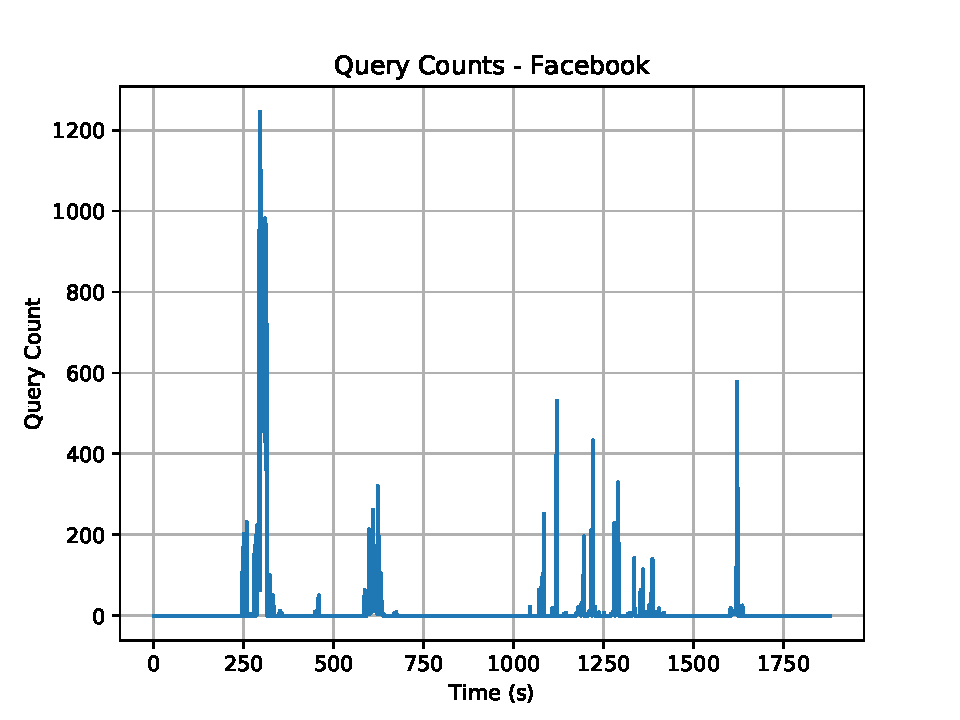
\includegraphics[width=0.45\textwidth]{graphics/ChangeOverTimeData}
    \caption{Sample Facebook Workload}
    \label{fig:sampleFacebook}
\end{figure}

\subsection{Session Identification}
\label{sec:backgroundSessionIdentification}
In traditional databases, a \textit{session} is defined as a connection between a user or an application, and the user~\cite{oracle9i}. Basically, every session has (1) a user or an application as the owner, (2) a start time where the user connects to the database, and (3) an end time where the user disconnects from the database.

This basic understanding of a session is not always enough for specific purposes such as prefetching predicted queries, or automatic query suggestion to the user. Yao \textit{et al.}~\cite{huang2006} define a session as a sequence of queries issued to the database by a user, or an application to achieve a \emph{certain task} where they adopt the some of the methods described from their previous work on web logs~\cite{huang2004dynamic}. 

The research on how to make use of database sessions using database query logs approximates to session identification in web search engine query logs, and it focuses on three approaches: (1) connection time approach, (2) time-out based approach, and (2) semantic segmentation of topics approach.

\tinysection{Connection time approach} This approach assumes that all the activity (and inactivity) belongs to one session as long as the user or the application is connected to the system. 

This approach is not suitable for mobiles systems since the database user sessions are local to the database. They do not correspond to the events of applications' connection and disconnection to the database.

Soikkeli \textit{et al.}~\cite{soikkeli2011diversity} say that even considering the time between launch and close of an application is not a reliable notion of an application usage session. Applications running in the foreground are visible to the user. Applications which are running in background are not visible to user even though he might have launched them before. 

% This approach is not suitable for mobiles systems since the applications tend to connect to the database when the operating system starts up, and the connection is closed when the operating system is turned off.

\tinysection{Timeout based approach} This approach is based on identifying a time-out value that is ideal for the given scenario to detect session boundaries. The queries that are issued between two boundaries belong to the same session. 

%\note{Our approach is not explored in the way that we did, but we can say that the closest approach to ours is timeout based approach. We will briefly discuss how the cited papers differs from our approach.}

\tinysection{Semantic segmentation based methods} This approach focuses on the content of the queries in order to understand the context change in the query workload~\cite{jones2008, huang2006, hagen2011}. The assumption is that, if two queries are semantically close to each other, they should be placed in the same session, and if there is a shift in the query interest, there should be session boundary between these queries. Naturally, this raises the question of \textit{what makes two queries similar?} The research on this question focuses on various motivations, such as database performance optimization~\cite{aouiche2006}, workload exploration~\cite{makiyama2015text}, and security applications~\cite{kul2016ettu}.

Yao \textit{et al.}~\cite{huang2006} report that sessions can be identified by studying change in information entropy. They use a language model which is chacterized by an order parameter and a threshhold parameter. The order parameter determines the granularity of the n-gram model which would be used to break the query log into smaller sequences of queries. The conditional probability of occurence of those sequences is calculated from the training data consisting of queries with sessions already identified beforehand. Using these probabilities, a running count of entropy is calculated for all sessions. The entropy parameter determines a threshold value at which a session can't accomodate any more new queries. These queries form part of another session and contribute of its entropy. If a sequence of queries has been observed to be occuring close to each other before, their entropy value will be low. This indicates presence of some kind of link between them and hence supports the case of them being in the same session. However, when a completely unrelated querie is being considered to be part of a particular session, the entropy value of the session will rise. The system would place the query in a different session. This approach is not dependent on time intervals. Even though this approach is very intuitive, it falls short of addressing specific issues in smartphone database sessions. As already described, there is no clear way to identify start and end of a session. As a result, it is not possible to obtain a training set of queries with sessions already labelled. Hence, this approach doesn't work for session identification in our case.

Hagen \textit{et al.}~\cite{hagen2011query} present an interesting approach to session identification which doesn't need simultaneous evaluation of all features of queries in the log. They propose the Cascade method which processes features in different steps each with increasing computational cost. When a computationally cheaper feature can make a reliable decision about session identificatio, features with higher computational cost and runtime are not processes. Additional features are evaluated only when computationally cheaper features don't provide a reliable decision. The Cascade method is designed on the assumption that time is not a good indicator of session boundaries. The scenario described in their work deals with online web searches. So, users stop working and resume their logical sessions after arbitarary amounts of time. 
They also refer to the state-of-the-art geometric method by Gayo-Avello ~\cite{gayo2009survey}. Like the geometric method, the cascade method uses the time and lexical similarity of queries to decide session boundaries. But for query pairs that are chronologically very close and lexically very different, the decision of the geometric method are not reliable. Hence, the cascade method invokes explicit semantic analysis and search result comparison to help decide session boundaries.  

%Although semantic segmentation of the queries performs very well for web log session identification, it may not always be practical in a database setting, both in traditional database systems, and in mobile databases. In traditional database systems, task oriented sessions where the user focuses on a single task can be identified with this approach, but when the user issues queries with different interests, this approach would fail to identify a sequence of queries that could be classified as a session. Similarly, in a mobile application, an activity can create a series of wide range of queries, which renders this approach inapplicable to identify sessions for a mobile application. 

\subsection{Session Similarity}

Once the the database user sessions have been identified, we need to identify sessions which perform similar logical activities.
A session can include one or more activities, and activities consist of a bag of queries as illustrated in Figure~\ref{fig:session}.
Exploring the similarities of sessions could be used to identify repeating patterns.

\begin{figure}[h!]
    \centering
    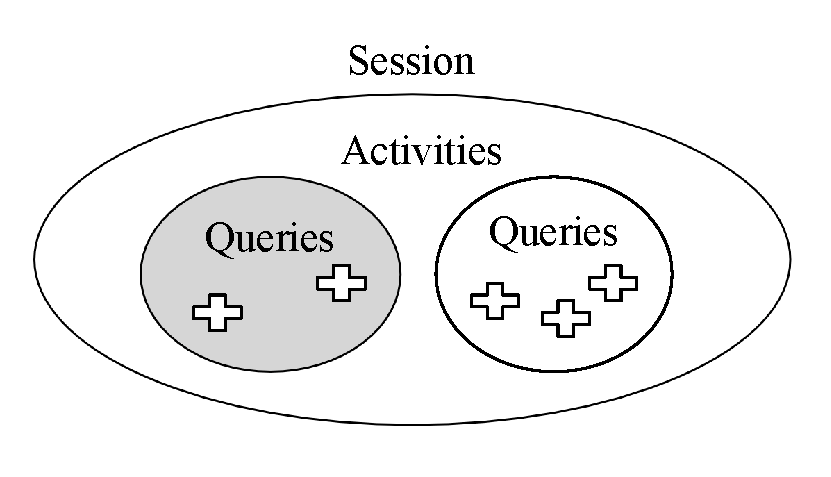
\includegraphics[width=0.45\textwidth]{graphics/Session}
    \caption{Session - Activity - Query relationship}
    \label{fig:session}
\end{figure}

Aligon \textit{et al.}~\cite{aligon2014similarity} report that there are 4 approaches in the literature for computing session similarity: (1) Edit-based approach, (2) Subsequence-based approach, (3) Log-based approach, and (4) Alignment-based approach.

Given two sessions \textit{A} and \textit{B}, and a treshold $\theta$, any approach given below first creates two sequences of placeholders for queries by comparing queries in both sessions to label each query pair that has a similarity score greater than $\theta$ as the same, and appoints distinct labels for other queries.

\tinysection{Edit-Based Approach} It finds the Levenshtein distance between the resulting sequences.

\tinysection{Subsequence-Based Approach} It computes the dice coefficient of n-grams of resulting sequences.

\tinysection{Log-Based Approach} It calculates the tf-idf value of the two sequences. This approach penalizes the queries that repeats a lot but is not distinctive.

\tinysection{Alignment-Based Approach} It considers the ordering of the queries along while comparing n-grams of resulting sequences. It finds the best alignments of n-grams to maximize the similarity.

\subsection{Mobile Workload Analysis}

There are various widely used benchmarking systems on traditional relational databases~\cite{council2008tpch, council2010tpcc, council2017tpcds, osdb2004}. 
DWEB~\cite{darmont2005dweb}, which is a data warehouse benchmark, also provides parameterization of data in terms of number of tables, and tuples; and parameterization of queries in terms of number of queries, and attributes in a query.
These benchmarks create scalable fixed data, and homogenous query workloads.
They focus on throughput and response time as the performance metric.

NoSQL database benchmarks~\cite{cooper2010YCSB, council2017tpcxiot}, on the other hand, appear to be more suitable to mobile database systems by providing support for configuring the query workload in terms of density of inserts, updates, deletes, and selects.
However, the queries are still pre-set in TPCx-IoT~\cite{council2017tpcxiot}. YCSB~\cite{cooper2010YCSB} only measures performance of key-value stores, and requires to be extended in order to process more complex queries.
Additionally, the workload created is still homogenous, and sequential.
 
There are also some mobile system database micro benchmarks such as AndroBench~\cite{liu2014application}, which was designed to evaluate the storage performance of the device, and not the database management system itself.

%and MobiGen~\cite{sabbir2009mobigen}

%Gray~\cite{gray1992benchmark} defines a ``good'' benchmark as one that provides \textit{relevance}, \textit{portability}, \textit{scalability}, and  \textit{simplicity}.
Even though a few of the mentioned benchmarks can satisfy 
%some of these
the requirements for mobile database systems, none of these benchmarks provide an accomplished mobile database management system evaluation, since there is a lack of understanding the behavior of mobile apps, and mobile operating systems as a class of database clients~\cite{kennedy2015pocket}.